\subsection{Calibration}
\label{sec:calibration}
In order to calibrate the detector the pulse generator was used to injected in
the pre-amplifier a known pulse. The oscilloscope was used to read the pulse
voltage that multiplied by the pre-amplifier capacitance gives the collected
charge as described in Section~\ref{sec:meas-appar}. The distribution on the MCA
was fitted with a Gaussian using the data taking software, the mean value is
then associated to a charge and the standard deviation used as uncertainty. This
procedure was performed for a set of input voltages and, due to time
restrictions, only for a gain value of 100. Figure~\ref{fig:calibration_fit}
shows the calculated collected charge as a function of the MCA channel number
with a linear fit superimposed. Figure~\ref{fig:calibration_raw} shows the
counts as a function of the MCA channel number.
\begin{figure}[!h]
  \centering
  \begin{subfigure}[t]{.48\linewidth}
    \includegraphics[width=\linewidth]{calibration_fit}
    \caption{Collected charge as a function of the multi-channel number}
    \label{fig:calibration_fit}
  \end{subfigure}
  \begin{subfigure}[t]{.48\linewidth}
    \includegraphics[width=\linewidth]{calibration_raw}
    \caption{Counts as a function of the multi-channel number}
    \label{fig:calibration_raw}
  \end{subfigure}
  \caption{}
  \label{fig:calibration}
\end{figure}

\begin{figure}[!h]
  \centering
  \begin{subfigure}[t]{.48\linewidth}
    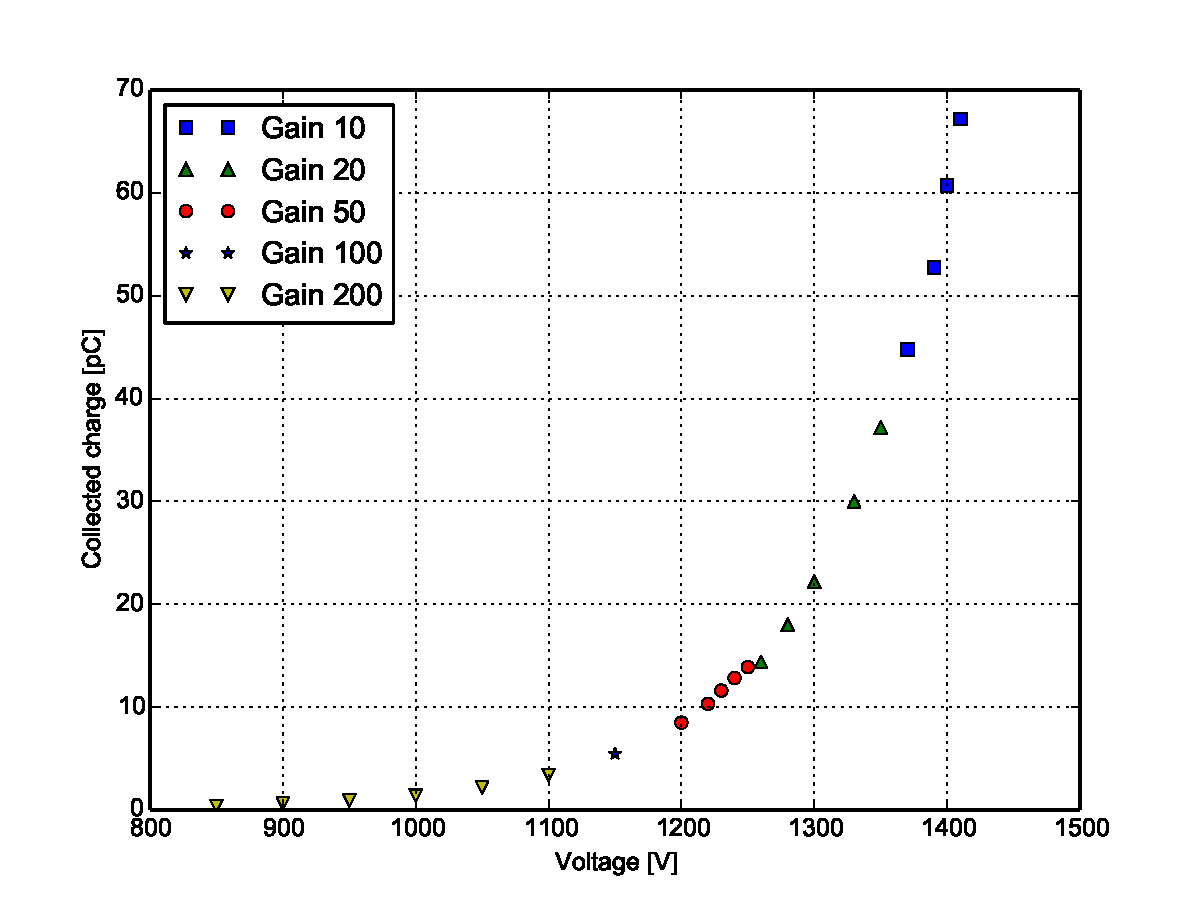
\includegraphics[width=\linewidth]{charge_vs_voltage}
    \caption{}
    \label{fig:charge_vs_voltage}
  \end{subfigure}
  \begin{subfigure}[t]{.48\linewidth}
    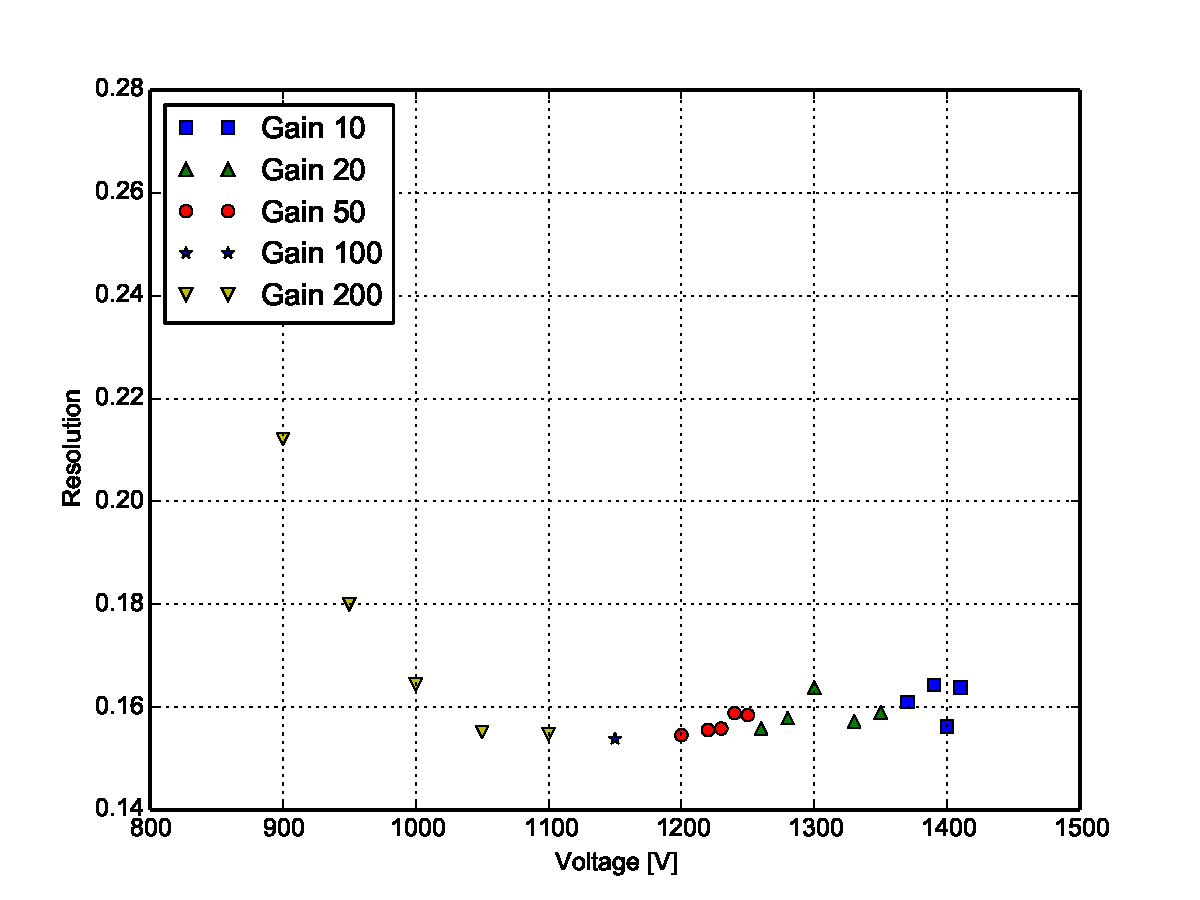
\includegraphics[width=\linewidth]{resolution_vs_voltage}
    \caption{}
    \label{fig:resolution_vs_voltage}
  \end{subfigure}
  \caption{}
  \label{fig:results}
\end{figure}
%%% Local Variables:
%%% mode: latex
%%% TeX-master: "prop_counter"
%%% End:
